Our motion segmentation algorithm is based on \emph{change-point detection}. A
change-point is an abrupt variation in the generative parameters of sequential
data. An efficient Bayesian on-line method for detecting change-points has been
independently proposed by Adams and MacKay~\cite{adams07bayesian} and by
Fearnhead and Liu~\cite{fearnhead07online}. In the following, we first present
this method in general and then show how we apply it to the problem of
segmenting motion data.

\subsection{Change-Point Detection}
Suppose we are given a time-dependent sequence of observations $\mathbf{z}_1,
\mathbf{z}_2, \dots,\mathbf{z}_T$, where the $\mathbf{z}_t$ can be scalars or
vectors. Our goal is to find segments $s_1,s_2,\dots,s_N$ with
$s_n=[\mathbf{z}_{b_n},\dots,\mathbf{z}_{e_n}]$, where $e_n > b_n$ and
$b_n = e_{n-1}+1$ for $n=1,\dots,N$. We assume that all data points
$\mathbf{z}_{b_n},\dots,\mathbf{z}_{e_n}$ of a segment $s_n$ are independently
and identically distributed (i.i.d.) according to a parameterized statistical
model \mbox{$p(\mathbf{z}\mid \boldsymbol{\eta}_n)$}. The parameter vectors
$\boldsymbol{\eta}_1,\dots \boldsymbol{\eta}_N$ are also assumed to be i.i.d.
The computation of the segments is done on-line, i.e., at each time step $t$ a
decision is made whether $\mathbf{z}_t$ is added to the current segment
$s_n=[\mathbf{z}_{b_n},\dots,\mathbf{z}_{t-1}]$ or a new segment is started. As
shown above, we denote the length of the current segment as $r_t$. Thus, after
deciding on $\mathbf{z}_t$, we have either $r_t=r_{t-1}+1$ or $r_t=0$ in case we
start a new segment.

To determine whether time step $t$ is a change-point, we analyze the posterior
distribution of the segment length conditioned on the data observed so far,
i.e. $p(r_t\mid \mathbf{z}_{1:t})$. Using the product rule, this filtering
distribution can be written as

\begin{equation}
\label{eqn:posterior}
p(r_t\mid \mathbf{z}_{1:t})\propto p(r_t,\mathbf{z}_{1:t}).
\end{equation}

The joint distribution in \eqref{eqn:posterior} can be further expressed as

\begin{eqnarray}
\label{eqn:joint}
p(r_t,\mathbf{z}_{1:t})\hspace{-0.2cm}&=& \hspace{-0.35cm}\sum_{r_{t-1}}p(r_t,
r_{t-1},\mathbf{z}_{1:t})\nonumber\\
&=&\hspace{-0.35cm}\sum_{r_{t-1}}p(r_t,\mathbf{z}_t\mid r_{t-1},
\mathbf{z}_{1:t-1})p(r_{t-1},\mathbf{z}_{1:t-1})\nonumber\\
&=&\hspace{-0.35cm}\sum_{r_{t-1}}p(r_t\mid r_{t-1})p(\mathbf{z}_t\mid r_{t-1},
\mathbf{z}_{1:t-1})p(r_{t-1},\mathbf{z}_{1:t-1}).
\end{eqnarray}

The right-hand side of \eqref{eqn:joint} consists of three terms: the
\emph{transition probability} $p(r_t\mid r_{t-1})$ of the Markov chain formed by
$r_1,r_2,\dots,r_t$, the \emph{predictive distribution}
$p(\mathbf{z}_t\mid r_{t-1},\mathbf{z}_{1:t-1})$, and the posterior
$p(r_{t-1},\mathbf{z}_{1:t-1})$ from the previous time step. We have exploited
Markov assumption for the simplifications in \eqref{eqn:joint}.
%Fig.\ref{fig:model} illustrates \eqref{eqn:joint} with a graphical model.

%\begin{figure}[t]
%\centering
%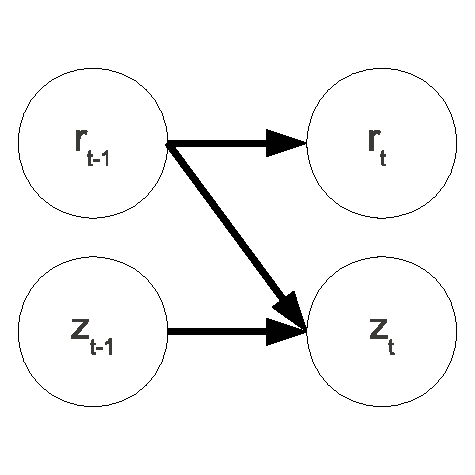
\includegraphics[width=0.5\columnwidth]{fig/model.eps}
%\caption{Graphical model representation of the joint posterior
%  $p(r_t,\mathbf{z}_{1:t})$.}
%\label{fig:model}
%\end{figure}

As there are only two possible successor states for $r_t$, namely
\mbox{$r_{t-1}+1$} or $0$, we can model the transition probability using
statistical survival analysis, i.e., the segment length can
either ``survive'' or ``die''. To do this, we define a \emph{survival function}
$S(t)$ as the probability that the current segment is still alive after time
step $t$. The complement of $S$ is usually named the
\emph{lifetime distribution function} $F(t)= 1- S(t)$ and its temporal
derivative $f(t)$ is denoted the \emph{event rate}. Finally, the
\emph{hazard function} $h(t)$ is defined as the event rate conditioned on the
survival of the segment at time $t$, i.e.

\begin{equation}
\label{eqn:hazardfunc}
h(t) = \frac{f(t)}{S(t)} = \frac{f(t)}{1 - F(t)}.
\end{equation}

Intuitively, $h(t)$ represents the probability that the segment dies exactly at
the current time instant $t$. We can use $h(t)$ to model the transition
probability as

\begin{equation}
\label{eqn:transprob}
p(r_t\mid r_{t-1}) = \left\{
\begin{array}{l l}
h(r_{t-1}+1) & \quad \text{if $r_t=0$ }\\
1 - h(r_{t-1}+1) & \quad \text{if $r_t=r_{t-1}+1$}\\
0 & \quad \text{otherwise}.
\end{array} \right.
\end{equation}

A common approach is to model $S(t)$ as an exponential function
$S(t)=\exp(-\lambda t)$ with some given rate parameter $\lambda$. Then, the
hazard function turns into

\begin{equation}
\label{eqn:hazardexp}
h(t) = \frac{\lambda\exp(-\lambda t)}{\exp(-\lambda t)} = \lambda.
\end{equation}

Thus, the hazard rate is constant and the process is ``memoryless''.
%Fig.~\ref{fig:transition} shows an example of possible transitions
%from $r_{t-1}$ to $r_{t+1}$.

%\begin{figure}[t]
%\centering
%\begin{tikzpicture}[scale=0.45]
%\tikzstyle{every node} = [rectangle,draw=blue!50,fill=blue!20,thick,
%inner sep=0pt,minimum size=6mm]
%\node (a) at (-4, 2) {$r_{t-1}=0$};
%\node (b) at (-4, 0) {$r_{t-1}=1$};
%\node (c) at (-4, -2) {$r_{t-1}=2$};
%\node (d) at (0, 2) {$r_t=0$};
%\node (e) at (0, 0) {$r_t=1$};
%\node (f) at (0, -2) {$r_t=2$};
%\node (g) at (4, 2) {$r_{t+1}=0$};
%\node (h) at (4, 0) {$r_{t+1}=1$};
%\node (i) at (4, -2) {$r_{t+1}=2$};
%\draw [->,thick] (a) -- (d);
%\draw [->,thick] (a) -- (e);
%\draw [->,thick] (b) -- (d);
%\draw [->,thick] (b) -- (f);
%\draw [->,thick] (c) -- (d);
%\draw [->,thick] (d) -- (h);
%\draw [->,thick] (d) -- (g);
%\draw [->,thick] (e) -- (i);
%\draw [->,thick] (e) -- (g);
%\draw [->,thick] (f) -- (g);
%\end{tikzpicture}
%\caption{Example of possible transitions from $r_{t-1}$ to $r_{t+1}$.}
%\label{fig:transition}
%\end{figure}

For the computation of the predictive distribution, we can make it dependent
only on the last data point $\mathbf{z}_{t-1}$ since we are doing a sequential
update of the parameters. Thus, it can be expressed as $p(\mathbf{z}_t
\mid r_{t-1}, \mathbf{z}_{t-1})$. We finally
introduce the model parameters $\boldsymbol{\eta}^{r_{t-1}}$ that are learned
on the current segment and compute the predictive distribution by marginalizing
them out, i.e.

\begin{equation}
\label{eqn:preddistr}
p(\mathbf{z}_t\mid r_{t-1},\mathbf{z}_{t-1},\boldsymbol{\psi}^{r_{t-1}})
= \phantom{aaaaaaaaaaaaaaaaaaaaaaaaaaaaaa}\nonumber
\end{equation}
\begin{equation}
 \phantom{aaaaaaaa}\int_{\boldsymbol{\eta}^{r_{t-1}}}
p(\mathbf{z}_t\mid\boldsymbol{\eta}^{r_{t-1}})p(\boldsymbol{\eta}^{r_{t-1}}\mid
r_{t-1},\mathbf{z}_{t-1},\boldsymbol{\psi}^{r_{t-1}})
d\boldsymbol{\eta}^{r_{t-1}}.
\end{equation}

Here, we have added the prior hyperparameters $\boldsymbol{\psi}^{r_{t-1}}$ for
completeness. The integral in \eqref{eqn:preddistr} can be solved analytically
if we model the prior of the parameter vector $\boldsymbol{\eta}^{r_{t-1}}$ as a
conjugate to the probability density function $p(\mathbf{z}_t\mid
\boldsymbol{\eta}^{r_{t-1}})$. Otherwise, this leads to expensive numerical
computations. When the terms inside the integral are conjugate models, the
marginal distribution is usually a function of the hyperparameters
$\boldsymbol{\psi}^{r_{t-1}}$ which can be updated iteratively as data arrives.

\subsection{Complexity and Approximate Inference}
In order to exactly infer the positions of all change-points until time $t$, we
need to compute and store $p(r_t\mid \mathbf{z}_{1:t})$ for $t$ and all previous
time steps. We can then get the Maximum A Posteriori (MAP) estimate of the
sequence of segment lengths using the on-line Viterbi
algorithm of~\cite{fearnhead07online}.

Regarding complexity, if we have processed $n$ data points, the storage of the
full posterior distribution has a memory cost of $O(n^2)$ and $O(n)$
computational cost. This might be prohibitive for huge datasets. For this
reason, the distribution has to be approximated. A simple way sketched
in~\cite{adams07bayesian} is to discard values where the distribution is
significantly low, i.e., lower than a given threshold. However, as we want to
accurately estimate our distribution and control the computational costs, we use
a \emph{particle filter}. The state-space of $r_t$ being discrete and the number
of successor states being small, we can evaluate all the possible descendants of
$r_t$. Indeed, if $r_t$ takes $k$ possible values, $r_{t+1}$ will take $k+1$
possible values. At each time step $t$, we approximate the posterior
distribution with a set $\{r_t^{(i)},\boldsymbol{\psi}^{r_{t-1},(i)}\}_{i=1}^M$ of
$M$ particles weighted by $\{w_t^{(i)}\}_{i=1}^M$ with

\begin{equation}
\label{eqn:weight}
w_t^{(i)} \propto p(\mathbf{z}_t\mid r_{t-1}^{(i)},\mathbf{z}_{t-1},
\boldsymbol{\psi}^{r_{t-1},(i)}).
\end{equation}

In order to limit the number of particles at each time step, we use the
Stratified Optimal Re-sampling (SOR) presented in~\cite{fearnhead07online},
whenever $M$ gets bigger than our particles number limit $P$.

Using this method reduces the memory costs to $O(n)$ and the computational costs
to $O(1)$, i.e. constant run-time. We also notice that this particle filter is
Rao-Blackwellized~\cite{casella96rao} and has thus a lower variance since the
sampling space of the state is reduced to $r_t$ and the rest is marginalized out.

\subsection{Application to Motion Data Segmentation}
In our particular case, data comes from an IMU and we consider accelerations in
the $x,y$ axes and the $yaw$ rate, with $x$ pointing forward, $y$ on the left,
and $z$ upward. We can safely assume that an IMU measurement $\mathbf{z}_t$
arises from a multivariate normal distribution with mean $\boldsymbol{\mu}_n$
and covariance matrix $\boldsymbol{\Sigma}_n$ for segment $s_n$. The parameter
vector for segment $r_t$ is thus $\boldsymbol{\eta}^{r_{t}}=
\{\boldsymbol{\mu}^{r_{t}},\boldsymbol{\Sigma}^{r_{t}}\}$. In order to solve
the integral in (\ref{eqn:preddistr}) analytically, we model the parameter prior
as a normal-Wishart distribution which is conjugate to the multivariate
Gaussian. This distribution has four hyperparameters
$\boldsymbol{\psi}^{r_{t}}=\{\kappa^{r_{t}},\boldsymbol{\rho}^{r_{t}},
\nu^{r_{t}},\boldsymbol{\Lambda}^{r_{t}}\}$ that can be updated iteratively
as a new data point $\mathbf{z}_t$ arrives with:

\begin{eqnarray}
\label{eqn:hyperupdate}
\kappa^{r_{t}}&=&\kappa^{r_{t-1}}+1\nonumber\\
\boldsymbol{\rho}^{r_{t}}&=&\frac{\kappa^{r_{t-1}}\;
\boldsymbol{\rho}^{r_{t-1}}+\mathbf{z}_t}{\kappa^{r_{t-1}}+1}\nonumber\\
\nu^{r_{t}}&=&\nu^{r_{t-1}}+1\nonumber\\
\boldsymbol{\Lambda}^{r_{t}}&=&\boldsymbol{\Lambda}^{r_{t-1}}+
\frac{\kappa^{r_{t-1}}}{\kappa^{r_{t-1}} + 1}
(\mathbf{z}_t - \boldsymbol{\rho}^{r_{t-1}})
(\mathbf{z}_t - \boldsymbol{\rho}^{r_{t-1}})^\intercal.
\end{eqnarray}

In case we start a new segment and $r_t=0$, the hyperparameters are fixed to
some prior values $\boldsymbol{\psi}_0=\{\kappa_0,\boldsymbol{\rho}_0,\nu_0,
\boldsymbol{\Lambda}_0\}$.

From (\ref{eqn:hyperupdate}), we can express the parameters of the resulting
multivariate normal distribution in \eqref{eqn:preddistr} as

\begin{eqnarray}
\label{eqn:ssmvn}
\boldsymbol{\mu}^{r_{t}}&=&\boldsymbol{\rho}^{r_{t}}\nonumber\\
\boldsymbol{\Sigma}^{r_{t}}&=&(\boldsymbol{\Lambda}^{r_{t}})^{-1}/\kappa^{r_{t}}.
\end{eqnarray}

Finally, for the computation of the predictive distribution in
\eqref{eqn:preddistr}, we approximate the multivariate normal distribution with
a Student's $t$-distribution which is known to be more robust to outliers in
case of few data points. This distribution converges to the Gaussian when its
degrees of freedom go to infinity. We use the number of processed points as the
degrees of freedom for the distribution, so as to have a bigger variance at the
beginning.
